\documentclass[a4paper,12pt]{article}

%%% Работа с русским языком
\usepackage{cmap}					% поиск в PDF
\usepackage{mathtext} 				% русские буквы в формулах
\usepackage[T2A]{fontenc}			% кодировка
\usepackage[utf8]{inputenc}			% кодировка исходного текста
\usepackage[english,russian]{babel}	% локализация и переносы
\usepackage{comment}


%%% Дополнительная работа с математикой
\usepackage{amsfonts,amssymb,amsthm,mathtools} % AMS
\usepackage{amsmath}
\usepackage{icomma} % "Умная" запятая: $0,2$ --- число, $0, 2$ --- перечисление

%% Номера формул
%\mathtoolsset{showonlyrefs=true} % Показывать номера только у тех формул, на которые есть \eqref{} в тексте.

%% Шрифты
\usepackage{euscript}	 % Шрифт Евклид
\usepackage{mathrsfs} % Красивый матшрифт

\usepackage{extsizes} % Возможность сделать 14-й шрифт
\usepackage{geometry} % Простой способ задавать поля
\geometry{top=25mm}
\geometry{bottom=35mm}
\geometry{left=15mm}
\geometry{right=15mm}

\usepackage{chngcntr}
\usepackage{hyperref}

\usepackage{setspace} % Интерлиньяж
%\onehalfspacing % Интерлиньяж 1.5
%\doublespacing % Интерлиньяж 2
%\singlespacing % Интерлиньяж 1

\usepackage{lastpage} % Узнать, сколько всего страниц в документе.
\usepackage{soulutf8} % Модификаторы начертания

\counterwithin*{equation}{section}
\counterwithin*{equation}{subsection}



%% Свои команды
\DeclareMathOperator{\sgn}{\mathop{sgn}}

%% Перенос знаков в формулах (по Львовскому)
\newcommand*{\hm}[1]{#1\nobreak\discretionary{}
{\hbox{$\mathsurround=0pt #1$}}{}}

%%% Работа с картинками
\usepackage{graphicx}  % Для вставки рисунков
\graphicspath{{images/}{images2/}}  % папки с картинками
\setlength\fboxsep{3pt} % Отступ рамки \fbox{} от рисунка
\setlength\fboxrule{1pt} % Толщина линий рамки \fbox{}
\usepackage{wrapfig} % Обтекание рисунков и таблиц текстом

%%% Работа с таблицами
\usepackage{array,tabularx,tabulary,booktabs} % Дополнительная работа с таблицами
\usepackage{longtable}  % Длинные таблицы
\usepackage{multirow} % Слияние строк в таблице
\usepackage{graphicx}
\usepackage{fancyhdr}
\usepackage{hyperref}
\usepackage{booktabs}

\newcommand{\lt}{\left}
\newcommand{\rt}{\right}
\newcommand{\al}{\alpha}
\newcommand{\p}{\partial}
\newcommand{\D}{\Delta}
\newcommand{\fr}{\frac}
\newcommand{\dfr}{\dfrac}
\newcommand{\mbf}{\mathbf}
\newcommand{\ol}{\overline}
\newcommand{\bb}{\mathbb}
\newcommand{\om}{\Omega}
\newcommand{\Rw}{\Rightarrow}
\newcommand{\ve}{\varepsilon}
\newcommand{\vp}{\varphi}
\newcommand{\mc}{\mathcal}
\newcommand{\sg}{\sigma}


\pagestyle{fancy}
\fancyhf{}
\pagestyle{plain} % нумерация вкл.

\rhead{\today}
\lhead{Соколов Игорь, группа 573}

%%% Заголовок
\author{Соколов Игорь, группа 573}
\title{ДЗ №6 по Теории Вероятностей }
\date{\today}

\begin{document} % конец преамбулы, начало документа

\maketitle

\section{}
Предположим, что независимо $n$ раз кидается монетка с вероятностью выпадения
орла в каждом опыте равной $p \in [0.1, 0.9]$. Сколько раз нужно кинуть монетку, чтобы оценка ${\ol p(x)} = \fr{\sum_{k=1}^{n}x_k}{n}$ с вероятностью $\gamma \le 0.95$ отличалась от истинного значения $p$ не более, чем на величину $\delta = 0.01$? Применить неравенство Чебышева и предельную теорему, точность которой оценить неравенством Берри – Эссена. Сравнить результаты.

\textbf {Решение:}

\begin{enumerate}
\item

 {\it Неравенство Чебышёва:}
$$\bb P(|\xi - \bb E\xi|\geqslant x)\leqslant\fr{\bb D\xi}{x^2}$$

Применяем его для случайной величины ${\ol p(x)}$

$$\bb P(|{\ol p(x)} - p|\leqslant \delta)\geqslant 1 - \fr{\bb D\ol p(x)}{\delta^2}$$

Из условия независимости с.в. $x_1, x_2,\dots ,x_n$ имеем $\bb D \ol p(x) = \fr{\bb D x_k}{n} = \fr{p(1-p)}{n}$

Оценка $\ol p(x)$ с вероятностью $\gamma \geqslant 0.95$ гарантируется при 

$$\gamma \leqslant 1 - \fr{\bb D\ol p(x)}{\delta^2} = 1 - \fr{p(1-p)}{n\delta^2}$$

$$\Rightarrow n\geqslant \fr{p(1-p)}{\delta ^2(1 - \gamma)}$$

Так как величина $p(1 - p)$ достигает максимума при $p = 0.5$, данное неравенство заведомо выполнено при числе бросаний монетки 

$$n = \fr{0.5^2}{\delta^2(1-\gamma)}$$

\begin{enumerate}
\item {\it (ц.п.т) \it Если $\bb E(x_k^2) <\infty$, то $\dfr{\sum_{k =1}^{n}x_k - n\bb Ex_k}{\sqrt{n\bb Dx_k}} \xrightarrow{\text{d}} N(0,1)$, при $n\rightarrow\infty$}

\item {\it (неравенство Бэрри-Эссеена) Пусть дана бесконечная последовательность $X_n$ независимых одинаково распределённых случайных величин таких, что $\bb E(X_n) = 0, \bb E(X_n^2) = \sigma^2 > 0, \bb E(|X_n^3|) = \rho < \infty)$. Обозначим через $F_n$ распределение суммы вида $\fr{\sum\limits_{i = 1}^{n}X_i}{\sigma\sqrt{n}}$}. Тогда для всех $x$ и $n$ $$\rightarrow |F_n(x)- \mathcal{N}(x)|\leqslant \fr{C\rho}{\sigma^3\sqrt{n}}$$

Из ц.п.т. и неравенство Бэрри-Эссена получаем 
$$\sup\limits_{x}\lt| \bb P\lt(\sum\limits_{k = 1}^{n}\fr{x_k - np}{\sigma\sqrt{n}} < x\rt) - \mathcal{N}(x) \rt| \leqslant \fr{C\mu^3}{\sigma\sqrt{n}}$$

где $C\leqslant 0.7056,\quad \sigma ^2 = \bb D X_k = p(1-p),\quad \mathcal{N}(x) = \int\limits_{-\infty}^{x}\fr{e^{-\fr{t^2}{2}}}{\sqrt{2\pi}}dt$

$$\mu^3 = \bb E|x_k - p|^3 = p(1-p)^3 + (1-p)p^3 = \sigma^2(1 - 2\sigma^2)$$

Так как $\sum\limits_{k = 1}^{n}\fr{x_k - np}{\sigma\sqrt{n}} = \fr{\sqrt{n}}{\sigma}({\ol p(x) - p})$, то условие $|{\ol p(x)} - p|\leqslant \delta$ выполняется с вероятностью не менее

$$\mathcal{N}\lt(\fr{\delta\sqrt{n}}{\sigma}\rt) - \mc{N}\lt(-\fr{\delta\sqrt{n}}{\sigma}\rt) - \fr{2C\mu^3}{\sigma^3\sqrt{n}}$$

Разность $\mathcal{N}\lt(\fr{\delta\sqrt{n}}{\sigma}\rt) - \mc{N}\lt(-\fr{\delta\sqrt{n}}{\sigma}\rt)$ принимает наименьшее значение при максимальном $\sigma^2 = p(1-p)$, которое достигается при 	$p = 0.5$.

Также можно заметить, что наибольшее значение величины
$$\fr{\mu^3}{\sigma^3} = \fr{\sigma^2(1 - 2\sigma^2)}{\sg^3} = \fr{1}{\sg} - 2\sg$$ 

достигается при наименьшем возможном $\sg$, которое дает $p = 0.1$, откуда $\sg = 0.3$.

Таким образом, оценка для ${\ol p(x)}$ с вероятностью $\gamma > 0.95$ гарантируется при
$$\gamma \leqslant \mc{N}(2\delta\sqrt{n}) -  \mc{N}(-2\delta\sqrt{n}) - \fr{2\cdot0.7}{\sqrt{n}}\lt(\fr{1}{0.3} - 0.6\rt)$$

Найдем такой минимальный $n$, чтобы оценка $|{\ol p(x)} - p(x)|\leqslant \delta$ выполнялась.

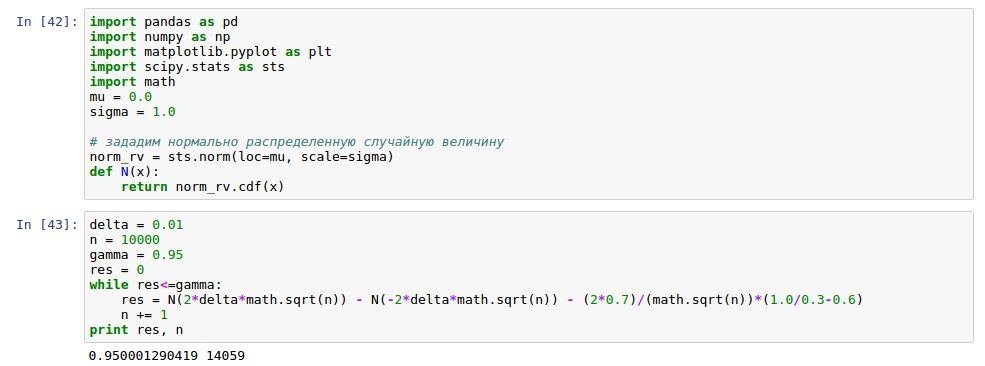
\includegraphics[width=\linewidth]{python.jpg}

То есть уже при $n = 14058$ имеем 
$$\mc{N}(2\delta\sqrt{n}) -  \mc{N}(-2\delta\sqrt{n} = 0.98228$$
$$\fr{2\cdot0.7}{\sqrt{n}}\lt(\fr{1}{0.3} - 0.6\rt) = 0.03227$$
$$\Rightarrow \gamma \geqslant 0.98228 - 0.03227 = 0.95000129 > 0.95 $$

$\Rightarrow |{\ol p(x)} - p(x)|\leqslant \delta$ выполняется.

Итог:

Сравнивая результаты, мы убедились, что предельная теорема дает более точные оценки и гарантирует нужную точность оценки для $p$ уже при при числе бросаний монетки $n = 14058$, в то время как
неравенство Чебышева — лишь при $n = 50000$.

	

\end{enumerate}
\end{enumerate}

\end{document} % конец документа

